\documentclass[11pt,a4paper]{article}
\usepackage[T1]{fontenc}
\usepackage[margin=25mm]{geometry}
\usepackage{amsmath,amssymb,amsthm}
\usepackage{microtype}
\usepackage{tikz}
\usepackage{url}

\newtheorem{conjecture}{Conjecture}
\newtheorem{theorem}{Theorem}
\newtheorem{lemma}[theorem]{Lemma}
\newtheorem{proposition}[theorem]{Proposition}
\theoremstyle{definition}
\newtheorem{definition}[theorem]{Definition}
\newtheorem*{remark}{Remark}
\setlength{\parindent}{0pt}
\setlength{\parskip}{0.45em}

\newcommand{\F}{\mathbb{F}}
\newcommand{\Tr}{\operatorname{Tr}}
\newcommand{\Res}{\operatorname{Res}}
\newcommand{\Aut}{\operatorname{Aut}}
\newcommand{\PSL}{\mathrm{PSL}}
\newcommand{\PGL}{\mathrm{PGL}}

% Colours and styles for the drawings generated by verify/Program.cs
\definecolor{ehink}{HTML}{1B2A4A}
\definecolor{ehred}{HTML}{D1495B}
\definecolor{ehgold}{HTML}{EDAE49}
\definecolor{ehteal}{HTML}{00798C}
\definecolor{ehplum}{HTML}{8E5EA2}
\definecolor{ehblue}{HTML}{30638E}
\definecolor{ehgreen}{HTML}{66A182}
\tikzset{
  ehespoke/.style   ={ehink,   line width=0.75pt, opacity=0.95},
  eheringA/.style   ={ehred,   line width=0.65pt, opacity=0.85},
  ehecrossAB/.style ={ehgold,  line width=0.55pt, opacity=0.80},
  ehecrossAC/.style ={ehteal,  line width=0.55pt, opacity=0.75},
  eheringB/.style   ={ehplum,  line width=0.60pt, opacity=0.80},
  ehecrossBC/.style ={ehblue,  line width=0.45pt, opacity=0.55},
  eheringC/.style   ={ehgreen, line width=0.60pt, opacity=0.80},
  ehegap0/.style    ={ehred,   line width=0.60pt, opacity=0.85},
  ehegap1/.style    ={ehgold,  line width=0.55pt, opacity=0.80},
  ehegap2/.style    ={ehteal,  line width=0.50pt, opacity=0.70},
  ehegap3/.style    ={ehblue,  line width=0.45pt, opacity=0.60},
  ehvertex/.style   ={circle, draw=ehink, fill=white, line width=0.8pt, inner sep=0pt, minimum size=4.2pt},
  ehcenter/.style   ={circle, draw=ehink, fill=ehink, line width=0.8pt, inner sep=0pt, minimum size=5.6pt},
}


\title{A Counterexample to the Equal Halves Conjecture\\[0.3em]
  \large The $\PSL(2,8)$ graph on 28 vertices}
\author{Claude Opus 5.5\\[0.2em]
  {\normalsize from a construction by M.~C.~Kao}}
\date{27/11/2026}

\begin{document}
\maketitle
\vspace{-1.5em}

\begin{abstract}
\noindent The Equal Halves Conjecture~\cite{G} asserts that every connected
vertex-transitive graph of even order has a partition of its vertex set into
two parts inducing connected isomorphic subgraphs. Ming-Chih Kao (@koolkao)
refuted it with eight graphs on 28 vertices, and the Lean~4 kernel checks the
refutation for one of them~\cite{K,LtS}. We explain that graph, the most
symmetric of the eight. It is a classical
graph: the valency-9 orbital graph of $\PSL(2,8)$ acting on 28 points, which
appears in work of Kutnar and Marušič~\cite{KM}. We give a short algebraic
description, explain why the involution argument of~\cite{G} does not apply,
and confirm the result by an independent computation.
\end{abstract}

\section{The conjecture}

All graphs are finite and simple. For $A\subseteq V(G)$, $G[A]$ is the induced
subgraph on~$A$.

\begin{conjecture}[Equal Halves~\cite{G}]
Every connected vertex-transitive graph $G$ of even order admits a partition
$V(G)=A\sqcup B$ into two nonempty sets such that $G[A]$ and $G[B]$ are
connected and isomorphic.
\end{conjecture}

The note~\cite{G} proves the conclusion whenever $G$ has an involutive
automorphism without fixed points, hence for every connected Cayley graph of
even order (left multiplication by an involution of the group). The Petersen
graph, the smallest vertex-transitive graph that is not a Cayley graph, also splits, into its outer 5-cycle and inner
pentagram. The conjecture was therefore open only for non-Cayley graphs.

\section{The graph $\Gamma$}

Let $\F=\F_8=\F_2[\alpha]/(\alpha^3+\alpha+1)$ and
$\Tr(x)=x+x^2+x^4$. Let $V$ be the set of monic irreducible quadratics
$q=x^2+bx+c\in\F[x]$. Such a $q$ has $b\neq0$ (otherwise it is a square), and
for $b\ne0$ it is irreducible if and only if $\Tr(c/b^2)=1$; hence $|V|=7\cdot4=28$.
For $q=x^2+bx+c$ and $q'=x^2+b'x+c'$ in $V$,
\[
  \Res(q,q') = (c+c')^2+(b+b')(bc'+b'c).
\]

\begin{lemma}\label{lem:rho}
For distinct $q,q'\in V$, the ratio $\rho(q,q')=\Res(q,q')/(bb')^2$ lies in
$\{\alpha,\alpha^2,\alpha^4\}$, the roots of $x^3+x+1$. It is invariant under
$\PGL(2,8)$, acting on $V$ through Möbius transformations of the roots.
\end{lemma}

\begin{proof}
Let $z,\bar z=z^8$ be the roots of $q$ and $w,\bar w$ those of $q'$, in
$\F_{64}$. Put $P=(z+w)(\bar z+\bar w)$ and $Q=(z+\bar w)(\bar z+w)$. Both are
fixed by $x\mapsto x^8$, so $P,Q\in\F^\times$. Moreover $\Res(q,q')=PQ$ and
$P+Q=(z+\bar z)(w+\bar w)=bb'\neq0$. Hence $\kappa=P/Q\in\F\setminus\{0,1\}$
and $\rho=\kappa/(1+\kappa)^2$. The element $y=\rho\kappa\in\F$ satisfies
$y^2+y=\rho^2$, so $\Tr(\rho)=\Tr(\rho^2)=0$. The nonzero elements of trace
$0$ are $\alpha,\alpha^2,\alpha^4$. Finally, $\kappa$ is the cross-ratio
$(z,\bar z;w,\bar w)$. Möbius maps with coefficients in $\F$ commute with
$x\mapsto x^8$ and preserve cross-ratios, and exchanging the roots of $q$ or
$q'$ replaces $\kappa$ by $1/\kappa$, which leaves $\rho$ unchanged.
\end{proof}

\begin{definition}
$\Gamma$ is the graph on $V$ in which $q\sim q'$ if and only if $\rho(q,q')=\alpha$.
\end{definition}

The three graphs $\Gamma_{\alpha}=\Gamma$, $\Gamma_{\alpha^2}$ and
$\Gamma_{\alpha^4}$ partition the edges of $K_{28}$. The map
$(b,c)\mapsto(b^2,c^2)$ sends $\rho$ to $\rho^2$, so it permutes them
cyclically and they are isomorphic. Over $\F_8$, $\PGL(2,8)=\PSL(2,8)$. This
group is transitive on $\F_{64}\setminus\F_8$, since the stabilizer of a point
is cyclic of order~9. Hence $\Gamma$ is vertex-transitive.

\begin{proposition}\label{prop:props}
\leavevmode
\begin{enumerate}\itemsep0pt
\item $\Gamma$ is connected and $9$-regular, with $126$ edges and diameter~$2$.
  Every edge lies in exactly two triangles. Two non-adjacent vertices have $2$
  or $4$ common neighbours ($126$ pairs each), so $\Gamma$ is not strongly
  regular. Its clique number is~$3$ and its independence number is~$7$.
\item The spectrum of $\Gamma$ is $9$, simple, and the three roots
  $2.604\ldots$, $-0.110\ldots$, $-3.494\ldots$ of $x^3+x^2-9x-1$, each of
  multiplicity~$9$.
\item $\Aut(\Gamma)=\PSL(2,8)$, of order $504$. The stabilizer of a vertex is
  dihedral of order~$18$, a maximal subgroup, so the action is primitive. The suborbits have lengths
  $1,9,9,9$, and they are exactly the classes of~$\rho$.
\item $\Gamma$ is the graph $X_1$ of Kutnar and Marušič~\cite[Table~2,
  Fig.~8]{KM}, who note that the three orbital graphs of $\PSL(2,8)$ on the
  cosets of $D_{18}$ are isomorphic. It is graph number $2659$ of the Holt--Royle
  census~\cite{HR} in Kao's numbering~\cite{K} (file
  \texttt{alltrans28\_k=09}, line~1186). Its complement is number $24010$.
\end{enumerate}
\end{proposition}

The proofs are by direct computation (Section~\ref{sec:proof}). The action is
well known in another guise. $\PSL(2,8)$ has index~$3$ in
$\mathrm{P\Gamma L}(2,8)\cong{}^2G_2(3)$, which acts $2$-transitively on the
same $28$ points, the points of the Ree unital of order~$3$~\cite{Lu}. The
field automorphism fuses the three orbital graphs into $K_{28}$.

\begin{proposition}\label{prop:invol}
Every involution of $\Aut(\Gamma)$ fixes exactly four vertices. Hence $\Gamma$
has no fixed-point-free involutive automorphism, and it is not a Cayley graph.
\end{proposition}

\begin{proof}
$\PSL(2,8)$ has a single class of $63$ involutions. The centralizer of an
involution $t$ has order~$8$, and $H=D_{18}$ contains $9$ involutions. So $t$
fixes $|C(t)|\cdot|t^G\cap H|/|H|=8\cdot9/18=4$ cosets of~$H$. A Cayley
structure would give a regular subgroup of order $28$, and its involutions
would have no fixed points.
\end{proof}

The $63$ fixed $4$-sets are the blocks of the Ree unital, a $2$-$(28,4,1)$
design. Proposition~\ref{prop:invol} puts $\Gamma$ beyond the reach of the
lemma of~\cite{G}.

\begin{figure}[t]
\centering
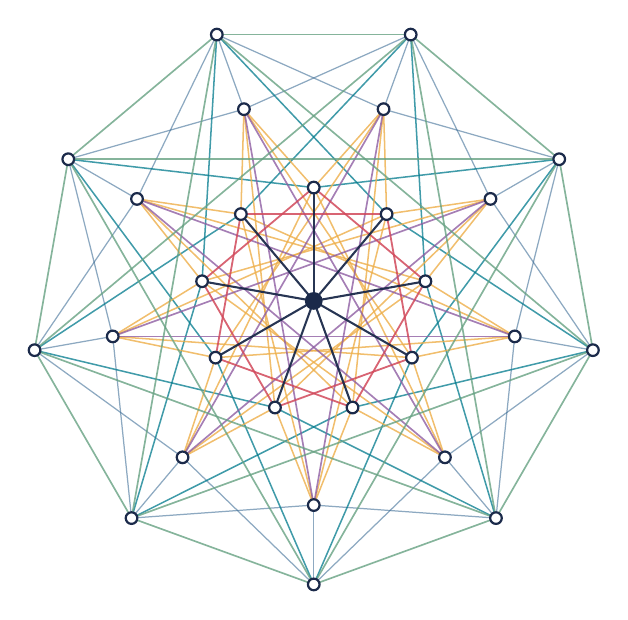
\begin{tikzpicture}[scale=3.6, line cap=round]
  % ninefold: generated by verify/Program.cs; edge classes spoke:9 ringA:9 ringC:18 ringB:9 crossAB:36 crossAC:18 crossBC:27
\draw[ehecrossBC] (-0.8660,0.5000) -- (-0.6235,0.3600);
\draw[ehecrossBC] (-0.8660,0.5000) -- (-0.7091,-0.1250);
\draw[ehecrossBC] (-0.8660,0.5000) -- (-0.2463,0.6766);
\draw[ehecrossBC] (-0.6235,0.3600) -- (-0.3420,0.9397);
\draw[ehecrossBC] (-0.6235,0.3600) -- (-0.9848,-0.1736);
\draw[ehecrossBC] (-0.0000,-0.7200) -- (-0.6428,-0.7660);
\draw[ehecrossBC] (-0.0000,-0.7200) -- (-0.0000,-1.0000);
\draw[ehecrossBC] (-0.0000,-0.7200) -- (0.6428,-0.7660);
\draw[ehecrossBC] (0.6235,0.3600) -- (0.3420,0.9397);
\draw[ehecrossBC] (0.6235,0.3600) -- (0.8660,0.5000);
\draw[ehecrossBC] (0.6235,0.3600) -- (0.9848,-0.1736);
\draw[ehecrossBC] (-0.6428,-0.7660) -- (-0.7091,-0.1250);
\draw[ehecrossBC] (-0.6428,-0.7660) -- (-0.4628,-0.5516);
\draw[ehecrossBC] (0.3420,0.9397) -- (-0.2463,0.6766);
\draw[ehecrossBC] (0.3420,0.9397) -- (0.2463,0.6766);
\draw[ehecrossBC] (0.4628,-0.5516) -- (-0.0000,-1.0000);
\draw[ehecrossBC] (0.4628,-0.5516) -- (0.9848,-0.1736);
\draw[ehecrossBC] (0.4628,-0.5516) -- (0.6428,-0.7660);
\draw[ehecrossBC] (0.7091,-0.1250) -- (0.8660,0.5000);
\draw[ehecrossBC] (0.7091,-0.1250) -- (0.9848,-0.1736);
\draw[ehecrossBC] (0.7091,-0.1250) -- (0.6428,-0.7660);
\draw[ehecrossBC] (-0.3420,0.9397) -- (-0.2463,0.6766);
\draw[ehecrossBC] (-0.3420,0.9397) -- (0.2463,0.6766);
\draw[ehecrossBC] (-0.9848,-0.1736) -- (-0.7091,-0.1250);
\draw[ehecrossBC] (-0.9848,-0.1736) -- (-0.4628,-0.5516);
\draw[ehecrossBC] (-0.0000,-1.0000) -- (-0.4628,-0.5516);
\draw[ehecrossBC] (0.8660,0.5000) -- (0.2463,0.6766);
\draw[ehecrossAC] (-0.8660,0.5000) -- (0.0000,0.4000);
\draw[ehecrossAC] (-0.8660,0.5000) -- (-0.3464,-0.2000);
\draw[ehecrossAC] (0.3464,-0.2000) -- (-0.0000,-1.0000);
\draw[ehecrossAC] (0.3464,-0.2000) -- (0.8660,0.5000);
\draw[ehecrossAC] (-0.6428,-0.7660) -- (0.1368,-0.3759);
\draw[ehecrossAC] (-0.6428,-0.7660) -- (-0.3939,0.0695);
\draw[ehecrossAC] (0.3420,0.9397) -- (0.3939,0.0695);
\draw[ehecrossAC] (0.3420,0.9397) -- (-0.2571,0.3064);
\draw[ehecrossAC] (0.0000,0.4000) -- (0.8660,0.5000);
\draw[ehecrossAC] (-0.3464,-0.2000) -- (-0.0000,-1.0000);
\draw[ehecrossAC] (-0.3420,0.9397) -- (0.2571,0.3064);
\draw[ehecrossAC] (-0.3420,0.9397) -- (-0.3939,0.0695);
\draw[ehecrossAC] (-0.9848,-0.1736) -- (-0.1368,-0.3759);
\draw[ehecrossAC] (-0.9848,-0.1736) -- (-0.2571,0.3064);
\draw[ehecrossAC] (0.2571,0.3064) -- (0.9848,-0.1736);
\draw[ehecrossAC] (-0.1368,-0.3759) -- (0.6428,-0.7660);
\draw[ehecrossAC] (0.1368,-0.3759) -- (0.9848,-0.1736);
\draw[ehecrossAC] (0.3939,0.0695) -- (0.6428,-0.7660);
\draw[ehecrossAB] (0.3464,-0.2000) -- (0.4628,-0.5516);
\draw[ehecrossAB] (0.3464,-0.2000) -- (0.7091,-0.1250);
\draw[ehecrossAB] (0.3464,-0.2000) -- (-0.7091,-0.1250);
\draw[ehecrossAB] (0.3464,-0.2000) -- (-0.2463,0.6766);
\draw[ehecrossAB] (-0.6235,0.3600) -- (0.1368,-0.3759);
\draw[ehecrossAB] (-0.6235,0.3600) -- (0.3939,0.0695);
\draw[ehecrossAB] (-0.6235,0.3600) -- (-0.3939,0.0695);
\draw[ehecrossAB] (-0.6235,0.3600) -- (-0.2571,0.3064);
\draw[ehecrossAB] (-0.0000,-0.7200) -- (0.2571,0.3064);
\draw[ehecrossAB] (-0.0000,-0.7200) -- (-0.1368,-0.3759);
\draw[ehecrossAB] (-0.0000,-0.7200) -- (0.1368,-0.3759);
\draw[ehecrossAB] (-0.0000,-0.7200) -- (-0.2571,0.3064);
\draw[ehecrossAB] (0.6235,0.3600) -- (0.2571,0.3064);
\draw[ehecrossAB] (0.6235,0.3600) -- (-0.1368,-0.3759);
\draw[ehecrossAB] (0.6235,0.3600) -- (0.3939,0.0695);
\draw[ehecrossAB] (0.6235,0.3600) -- (-0.3939,0.0695);
\draw[ehecrossAB] (0.0000,0.4000) -- (0.4628,-0.5516);
\draw[ehecrossAB] (0.0000,0.4000) -- (-0.2463,0.6766);
\draw[ehecrossAB] (0.0000,0.4000) -- (0.2463,0.6766);
\draw[ehecrossAB] (0.0000,0.4000) -- (-0.4628,-0.5516);
\draw[ehecrossAB] (-0.3464,-0.2000) -- (0.7091,-0.1250);
\draw[ehecrossAB] (-0.3464,-0.2000) -- (-0.7091,-0.1250);
\draw[ehecrossAB] (-0.3464,-0.2000) -- (0.2463,0.6766);
\draw[ehecrossAB] (-0.3464,-0.2000) -- (-0.4628,-0.5516);
\draw[ehecrossAB] (0.4628,-0.5516) -- (0.1368,-0.3759);
\draw[ehecrossAB] (0.4628,-0.5516) -- (-0.3939,0.0695);
\draw[ehecrossAB] (0.7091,-0.1250) -- (0.3939,0.0695);
\draw[ehecrossAB] (0.7091,-0.1250) -- (-0.2571,0.3064);
\draw[ehecrossAB] (0.2571,0.3064) -- (-0.7091,-0.1250);
\draw[ehecrossAB] (0.2571,0.3064) -- (0.2463,0.6766);
\draw[ehecrossAB] (-0.1368,-0.3759) -- (-0.2463,0.6766);
\draw[ehecrossAB] (-0.1368,-0.3759) -- (-0.4628,-0.5516);
\draw[ehecrossAB] (0.1368,-0.3759) -- (0.2463,0.6766);
\draw[ehecrossAB] (0.3939,0.0695) -- (-0.4628,-0.5516);
\draw[ehecrossAB] (-0.3939,0.0695) -- (-0.7091,-0.1250);
\draw[ehecrossAB] (-0.2571,0.3064) -- (-0.2463,0.6766);
\draw[eheringB] (-0.6235,0.3600) -- (0.4628,-0.5516);
\draw[eheringB] (-0.6235,0.3600) -- (0.7091,-0.1250);
\draw[eheringB] (-0.0000,-0.7200) -- (-0.2463,0.6766);
\draw[eheringB] (-0.0000,-0.7200) -- (0.2463,0.6766);
\draw[eheringB] (0.6235,0.3600) -- (-0.7091,-0.1250);
\draw[eheringB] (0.6235,0.3600) -- (-0.4628,-0.5516);
\draw[eheringB] (0.4628,-0.5516) -- (-0.2463,0.6766);
\draw[eheringB] (0.7091,-0.1250) -- (-0.7091,-0.1250);
\draw[eheringB] (0.2463,0.6766) -- (-0.4628,-0.5516);
\draw[eheringC] (-0.8660,0.5000) -- (-0.3420,0.9397);
\draw[eheringC] (-0.8660,0.5000) -- (-0.9848,-0.1736);
\draw[eheringC] (-0.8660,0.5000) -- (-0.0000,-1.0000);
\draw[eheringC] (-0.8660,0.5000) -- (0.8660,0.5000);
\draw[eheringC] (-0.6428,-0.7660) -- (-0.3420,0.9397);
\draw[eheringC] (-0.6428,-0.7660) -- (-0.9848,-0.1736);
\draw[eheringC] (-0.6428,-0.7660) -- (-0.0000,-1.0000);
\draw[eheringC] (-0.6428,-0.7660) -- (0.9848,-0.1736);
\draw[eheringC] (0.3420,0.9397) -- (-0.3420,0.9397);
\draw[eheringC] (0.3420,0.9397) -- (-0.9848,-0.1736);
\draw[eheringC] (0.3420,0.9397) -- (0.8660,0.5000);
\draw[eheringC] (0.3420,0.9397) -- (0.6428,-0.7660);
\draw[eheringC] (-0.3420,0.9397) -- (0.9848,-0.1736);
\draw[eheringC] (-0.9848,-0.1736) -- (0.6428,-0.7660);
\draw[eheringC] (-0.0000,-1.0000) -- (0.8660,0.5000);
\draw[eheringC] (-0.0000,-1.0000) -- (0.6428,-0.7660);
\draw[eheringC] (0.8660,0.5000) -- (0.9848,-0.1736);
\draw[eheringC] (0.9848,-0.1736) -- (0.6428,-0.7660);
\draw[eheringA] (0.3464,-0.2000) -- (0.2571,0.3064);
\draw[eheringA] (0.3464,-0.2000) -- (-0.1368,-0.3759);
\draw[eheringA] (0.0000,0.4000) -- (0.3939,0.0695);
\draw[eheringA] (0.0000,0.4000) -- (-0.3939,0.0695);
\draw[eheringA] (-0.3464,-0.2000) -- (0.1368,-0.3759);
\draw[eheringA] (-0.3464,-0.2000) -- (-0.2571,0.3064);
\draw[eheringA] (0.2571,0.3064) -- (-0.2571,0.3064);
\draw[eheringA] (-0.1368,-0.3759) -- (-0.3939,0.0695);
\draw[eheringA] (0.1368,-0.3759) -- (0.3939,0.0695);
\draw[ehespoke] (0.0000,0.0000) -- (0.3464,-0.2000);
\draw[ehespoke] (0.0000,0.0000) -- (0.0000,0.4000);
\draw[ehespoke] (0.0000,0.0000) -- (-0.3464,-0.2000);
\draw[ehespoke] (0.0000,0.0000) -- (0.2571,0.3064);
\draw[ehespoke] (0.0000,0.0000) -- (-0.1368,-0.3759);
\draw[ehespoke] (0.0000,0.0000) -- (0.1368,-0.3759);
\draw[ehespoke] (0.0000,0.0000) -- (0.3939,0.0695);
\draw[ehespoke] (0.0000,0.0000) -- (-0.3939,0.0695);
\draw[ehespoke] (0.0000,0.0000) -- (-0.2571,0.3064);
\node[ehcenter] at (0.0000,0.0000) {};
\node[ehvertex] at (-0.8660,0.5000) {};
\node[ehvertex] at (0.3464,-0.2000) {};
\node[ehvertex] at (-0.6235,0.3600) {};
\node[ehvertex] at (-0.0000,-0.7200) {};
\node[ehvertex] at (0.6235,0.3600) {};
\node[ehvertex] at (-0.6428,-0.7660) {};
\node[ehvertex] at (0.3420,0.9397) {};
\node[ehvertex] at (0.0000,0.4000) {};
\node[ehvertex] at (-0.3464,-0.2000) {};
\node[ehvertex] at (0.4628,-0.5516) {};
\node[ehvertex] at (0.7091,-0.1250) {};
\node[ehvertex] at (-0.3420,0.9397) {};
\node[ehvertex] at (-0.9848,-0.1736) {};
\node[ehvertex] at (0.2571,0.3064) {};
\node[ehvertex] at (-0.1368,-0.3759) {};
\node[ehvertex] at (-0.0000,-1.0000) {};
\node[ehvertex] at (0.1368,-0.3759) {};
\node[ehvertex] at (0.8660,0.5000) {};
\node[ehvertex] at (0.3939,0.0695) {};
\node[ehvertex] at (-0.3939,0.0695) {};
\node[ehvertex] at (-0.2571,0.3064) {};
\node[ehvertex] at (-0.7091,-0.1250) {};
\node[ehvertex] at (-0.2463,0.6766) {};
\node[ehvertex] at (0.2463,0.6766) {};
\node[ehvertex] at (0.9848,-0.1736) {};
\node[ehvertex] at (-0.4628,-0.5516) {};
\node[ehvertex] at (0.6428,-0.7660) {};

\end{tikzpicture}\hspace{0.6cm}%
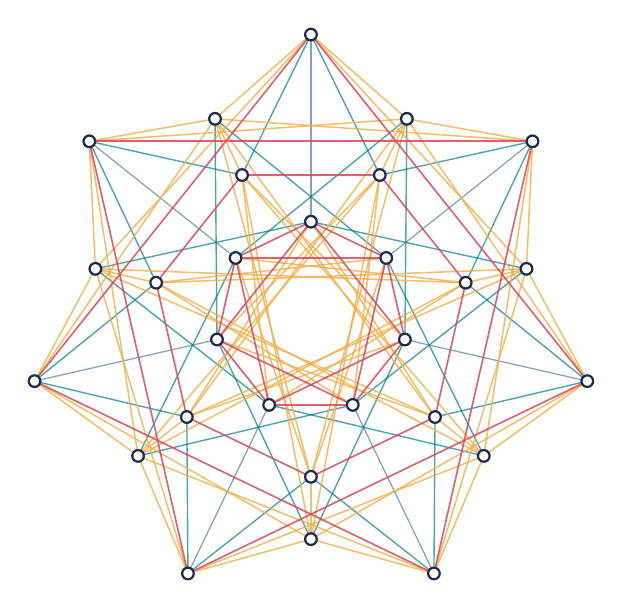
\begin{tikzpicture}[scale=3.6, line cap=round]
  % sevenfold: generated by verify/Program.cs; edge classes gap0:28 gap1:63 gap2:28 gap3:7
\draw[ehegap3] (0.0000,0.3400) -- (0.0000,1.0000);
\draw[ehegap3] (0.3315,-0.0757) -- (0.9749,-0.2225);
\draw[ehegap3] (0.4339,-0.9010) -- (0.1475,-0.3063);
\draw[ehegap3] (-0.7818,0.6235) -- (-0.2658,0.2120);
\draw[ehegap3] (-0.3315,-0.0757) -- (-0.9749,-0.2225);
\draw[ehegap3] (-0.1475,-0.3063) -- (-0.4339,-0.9010);
\draw[ehegap3] (0.7818,0.6235) -- (0.2658,0.2120);
\draw[ehegap2] (0.0000,0.3400) -- (-0.7604,0.1736);
\draw[ehegap2] (0.0000,0.3400) -- (0.7604,0.1736);
\draw[ehegap2] (0.2430,0.5045) -- (0.0000,1.0000);
\draw[ehegap2] (0.2430,0.5045) -- (0.7818,0.6235);
\draw[ehegap2] (0.3315,-0.0757) -- (-0.0000,-0.7800);
\draw[ehegap2] (0.3315,-0.0757) -- (0.3384,0.7028);
\draw[ehegap2] (0.5460,0.1246) -- (0.9749,-0.2225);
\draw[ehegap2] (0.5460,0.1246) -- (0.7818,0.6235);
\draw[ehegap2] (-0.0000,-0.5600) -- (0.4339,-0.9010);
\draw[ehegap2] (-0.0000,-0.5600) -- (-0.4339,-0.9010);
\draw[ehegap2] (-0.5460,0.1246) -- (-0.7818,0.6235);
\draw[ehegap2] (-0.5460,0.1246) -- (-0.9749,-0.2225);
\draw[ehegap2] (0.4339,-0.9010) -- (0.4378,-0.3492);
\draw[ehegap2] (-0.7818,0.6235) -- (-0.2430,0.5045);
\draw[ehegap2] (0.0000,1.0000) -- (-0.2430,0.5045);
\draw[ehegap2] (-0.3315,-0.0757) -- (-0.0000,-0.7800);
\draw[ehegap2] (-0.3315,-0.0757) -- (-0.3384,0.7028);
\draw[ehegap2] (0.9749,-0.2225) -- (0.4378,-0.3492);
\draw[ehegap2] (-0.1475,-0.3063) -- (-0.7604,0.1736);
\draw[ehegap2] (-0.1475,-0.3063) -- (0.6098,-0.4863);
\draw[ehegap2] (-0.6098,-0.4863) -- (-0.2658,0.2120);
\draw[ehegap2] (-0.6098,-0.4863) -- (0.1475,-0.3063);
\draw[ehegap2] (0.2658,0.2120) -- (-0.3384,0.7028);
\draw[ehegap2] (0.2658,0.2120) -- (0.6098,-0.4863);
\draw[ehegap2] (-0.4378,-0.3492) -- (-0.9749,-0.2225);
\draw[ehegap2] (-0.4378,-0.3492) -- (-0.4339,-0.9010);
\draw[ehegap2] (0.7604,0.1736) -- (0.1475,-0.3063);
\draw[ehegap2] (-0.2658,0.2120) -- (0.3384,0.7028);
\draw[ehegap1] (0.0000,0.3400) -- (-0.4378,-0.3492);
\draw[ehegap1] (0.0000,0.3400) -- (0.4378,-0.3492);
\draw[ehegap1] (0.2430,0.5045) -- (-0.3315,-0.0757);
\draw[ehegap1] (0.2430,0.5045) -- (-0.6098,-0.4863);
\draw[ehegap1] (0.2430,0.5045) -- (-0.0000,-0.7800);
\draw[ehegap1] (0.2430,0.5045) -- (0.1475,-0.3063);
\draw[ehegap1] (0.2430,0.5045) -- (0.3384,0.7028);
\draw[ehegap1] (0.3315,-0.0757) -- (-0.4378,-0.3492);
\draw[ehegap1] (0.3315,-0.0757) -- (-0.2430,0.5045);
\draw[ehegap1] (0.5460,0.1246) -- (-0.1475,-0.3063);
\draw[ehegap1] (0.5460,0.1246) -- (-0.6098,-0.4863);
\draw[ehegap1] (0.5460,0.1246) -- (-0.7604,0.1736);
\draw[ehegap1] (0.5460,0.1246) -- (0.7604,0.1736);
\draw[ehegap1] (0.5460,0.1246) -- (-0.2658,0.2120);
\draw[ehegap1] (-0.0000,-0.5600) -- (0.2658,0.2120);
\draw[ehegap1] (-0.0000,-0.5600) -- (-0.0000,-0.7800);
\draw[ehegap1] (-0.0000,-0.5600) -- (-0.2658,0.2120);
\draw[ehegap1] (-0.0000,-0.5600) -- (0.3384,0.7028);
\draw[ehegap1] (-0.0000,-0.5600) -- (-0.3384,0.7028);
\draw[ehegap1] (-0.5460,0.1246) -- (0.2658,0.2120);
\draw[ehegap1] (-0.5460,0.1246) -- (-0.7604,0.1736);
\draw[ehegap1] (-0.5460,0.1246) -- (0.7604,0.1736);
\draw[ehegap1] (-0.5460,0.1246) -- (0.1475,-0.3063);
\draw[ehegap1] (-0.5460,0.1246) -- (0.6098,-0.4863);
\draw[ehegap1] (0.4339,-0.9010) -- (-0.6098,-0.4863);
\draw[ehegap1] (0.4339,-0.9010) -- (-0.0000,-0.7800);
\draw[ehegap1] (0.4339,-0.9010) -- (0.7604,0.1736);
\draw[ehegap1] (0.4339,-0.9010) -- (0.6098,-0.4863);
\draw[ehegap1] (-0.7818,0.6235) -- (-0.6098,-0.4863);
\draw[ehegap1] (-0.7818,0.6235) -- (-0.7604,0.1736);
\draw[ehegap1] (-0.7818,0.6235) -- (0.3384,0.7028);
\draw[ehegap1] (-0.7818,0.6235) -- (-0.3384,0.7028);
\draw[ehegap1] (0.0000,1.0000) -- (-0.7604,0.1736);
\draw[ehegap1] (0.0000,1.0000) -- (0.7604,0.1736);
\draw[ehegap1] (0.0000,1.0000) -- (0.3384,0.7028);
\draw[ehegap1] (0.0000,1.0000) -- (-0.3384,0.7028);
\draw[ehegap1] (-0.3315,-0.0757) -- (0.4378,-0.3492);
\draw[ehegap1] (0.9749,-0.2225) -- (-0.0000,-0.7800);
\draw[ehegap1] (0.9749,-0.2225) -- (0.7604,0.1736);
\draw[ehegap1] (0.9749,-0.2225) -- (0.3384,0.7028);
\draw[ehegap1] (0.9749,-0.2225) -- (0.6098,-0.4863);
\draw[ehegap1] (-0.1475,-0.3063) -- (-0.2430,0.5045);
\draw[ehegap1] (0.7818,0.6235) -- (0.7604,0.1736);
\draw[ehegap1] (0.7818,0.6235) -- (0.3384,0.7028);
\draw[ehegap1] (0.7818,0.6235) -- (-0.3384,0.7028);
\draw[ehegap1] (0.7818,0.6235) -- (0.6098,-0.4863);
\draw[ehegap1] (-0.6098,-0.4863) -- (-0.4378,-0.3492);
\draw[ehegap1] (-0.6098,-0.4863) -- (-0.9749,-0.2225);
\draw[ehegap1] (-0.6098,-0.4863) -- (-0.4339,-0.9010);
\draw[ehegap1] (-0.4378,-0.3492) -- (0.7604,0.1736);
\draw[ehegap1] (-0.4378,-0.3492) -- (0.3384,0.7028);
\draw[ehegap1] (-0.0000,-0.7800) -- (-0.2430,0.5045);
\draw[ehegap1] (-0.0000,-0.7800) -- (-0.9749,-0.2225);
\draw[ehegap1] (-0.0000,-0.7800) -- (-0.4339,-0.9010);
\draw[ehegap1] (0.4378,-0.3492) -- (-0.7604,0.1736);
\draw[ehegap1] (0.4378,-0.3492) -- (-0.3384,0.7028);
\draw[ehegap1] (0.4378,-0.3492) -- (0.6098,-0.4863);
\draw[ehegap1] (-0.2430,0.5045) -- (-0.3384,0.7028);
\draw[ehegap1] (-0.2430,0.5045) -- (0.6098,-0.4863);
\draw[ehegap1] (-0.7604,0.1736) -- (-0.9749,-0.2225);
\draw[ehegap1] (-0.7604,0.1736) -- (-0.4339,-0.9010);
\draw[ehegap1] (-0.3384,0.7028) -- (-0.9749,-0.2225);
\draw[ehegap1] (0.6098,-0.4863) -- (-0.4339,-0.9010);
\draw[ehegap0] (0.0000,0.3400) -- (0.3315,-0.0757);
\draw[ehegap0] (0.0000,0.3400) -- (-0.3315,-0.0757);
\draw[ehegap0] (0.0000,0.3400) -- (0.2658,0.2120);
\draw[ehegap0] (0.0000,0.3400) -- (-0.2658,0.2120);
\draw[ehegap0] (0.2430,0.5045) -- (0.5460,0.1246);
\draw[ehegap0] (0.2430,0.5045) -- (-0.2430,0.5045);
\draw[ehegap0] (0.3315,-0.0757) -- (-0.1475,-0.3063);
\draw[ehegap0] (0.3315,-0.0757) -- (0.2658,0.2120);
\draw[ehegap0] (0.3315,-0.0757) -- (0.1475,-0.3063);
\draw[ehegap0] (0.5460,0.1246) -- (0.4378,-0.3492);
\draw[ehegap0] (-0.0000,-0.5600) -- (-0.4378,-0.3492);
\draw[ehegap0] (-0.0000,-0.5600) -- (0.4378,-0.3492);
\draw[ehegap0] (-0.5460,0.1246) -- (-0.4378,-0.3492);
\draw[ehegap0] (-0.5460,0.1246) -- (-0.2430,0.5045);
\draw[ehegap0] (0.4339,-0.9010) -- (0.7818,0.6235);
\draw[ehegap0] (0.4339,-0.9010) -- (-0.9749,-0.2225);
\draw[ehegap0] (-0.7818,0.6235) -- (0.7818,0.6235);
\draw[ehegap0] (-0.7818,0.6235) -- (-0.4339,-0.9010);
\draw[ehegap0] (0.0000,1.0000) -- (0.9749,-0.2225);
\draw[ehegap0] (0.0000,1.0000) -- (-0.9749,-0.2225);
\draw[ehegap0] (-0.3315,-0.0757) -- (-0.1475,-0.3063);
\draw[ehegap0] (-0.3315,-0.0757) -- (-0.2658,0.2120);
\draw[ehegap0] (-0.3315,-0.0757) -- (0.1475,-0.3063);
\draw[ehegap0] (0.9749,-0.2225) -- (-0.4339,-0.9010);
\draw[ehegap0] (-0.1475,-0.3063) -- (-0.2658,0.2120);
\draw[ehegap0] (-0.1475,-0.3063) -- (0.1475,-0.3063);
\draw[ehegap0] (0.2658,0.2120) -- (-0.2658,0.2120);
\draw[ehegap0] (0.2658,0.2120) -- (0.1475,-0.3063);
\node[ehvertex] at (0.0000,0.3400) {};
\node[ehvertex] at (0.2430,0.5045) {};
\node[ehvertex] at (0.3315,-0.0757) {};
\node[ehvertex] at (0.5460,0.1246) {};
\node[ehvertex] at (-0.0000,-0.5600) {};
\node[ehvertex] at (-0.5460,0.1246) {};
\node[ehvertex] at (0.4339,-0.9010) {};
\node[ehvertex] at (-0.7818,0.6235) {};
\node[ehvertex] at (0.0000,1.0000) {};
\node[ehvertex] at (-0.3315,-0.0757) {};
\node[ehvertex] at (0.9749,-0.2225) {};
\node[ehvertex] at (-0.1475,-0.3063) {};
\node[ehvertex] at (0.7818,0.6235) {};
\node[ehvertex] at (-0.6098,-0.4863) {};
\node[ehvertex] at (0.2658,0.2120) {};
\node[ehvertex] at (-0.4378,-0.3492) {};
\node[ehvertex] at (-0.0000,-0.7800) {};
\node[ehvertex] at (0.4378,-0.3492) {};
\node[ehvertex] at (-0.2430,0.5045) {};
\node[ehvertex] at (-0.7604,0.1736) {};
\node[ehvertex] at (0.7604,0.1736) {};
\node[ehvertex] at (-0.2658,0.2120) {};
\node[ehvertex] at (0.1475,-0.3063) {};
\node[ehvertex] at (0.3384,0.7028) {};
\node[ehvertex] at (-0.3384,0.7028) {};
\node[ehvertex] at (0.6098,-0.4863) {};
\node[ehvertex] at (-0.9749,-0.2225) {};
\node[ehvertex] at (-0.4339,-0.9010) {};

\end{tikzpicture}
\caption{Two drawings of $\Gamma$, each with a dihedral group of symmetries
inside $\Aut(\Gamma)$. \emph{Left:} the view from a vertex~$v$ (filled), with
the symmetries of its stabilizer $D_{18}$. The inner ring holds the $9$
neighbours of~$v$. The middle and outer rings hold the vertices with $4$ and
with $2$ common neighbours with~$v$. Edges: from~$v$ (ink), inside the inner ring
(red), inner--middle (gold), inner--outer (teal), inside the middle ring
(purple), middle--outer (grey-blue), inside the outer ring (green).
\emph{Right:} the four orbits of an element of order~$7$, with the symmetries of
its normalizer $D_{14}$. Edges join vertices in the same ring or in rings $1$,
$2$ or $3$ steps apart (red, gold, teal, blue).}
\label{fig:graph}
\end{figure}

\section{The counterexample}\label{sec:proof}

\begin{theorem}[Kao~\cite{K,LtS}]\label{thm:main}
There is no partition $V(\Gamma)=A\sqcup B$ with $\Gamma[A]\cong\Gamma[B]$,
connected or not. Hence $\Gamma$ is a connected vertex-transitive graph of even
order for which the Equal Halves Conjecture fails. So is its complement
$\overline\Gamma=\Gamma_{\alpha^2}\cup\Gamma_{\alpha^4}$, because
complementation preserves isomorphisms between induced subgraphs.
\end{theorem}

The proof is a finite computation. All three verifications below rest on the
following reduction.

\begin{lemma}\label{lem:tau}
If $\varphi\colon\Gamma[A]\to\Gamma[B]$ is an isomorphism, then
$\tau=\varphi\cup\varphi^{-1}$ is an involution of $V$ that swaps $A$ and $B$
and preserves adjacency inside each side. Hence $|A|=|B|=14$. Moreover, for
every statistic $s(v)$ computed inside the side of~$v$ (degree, number of
triangles, number of vertices at distance~$2$, \dots), the multisets
$\{s(v):v\in A\}$ and $\{s(v):v\in B\}$ are equal.
\end{lemma}

The involution $\tau$ need not be an automorphism of~$\Gamma$, because it may
break edges between $A$ and $B$. So Proposition~\ref{prop:invol} alone does not
settle the question.

\begin{enumerate}\itemsep2pt
\item[(i)] \emph{Lean certificate (Kao~\cite{LtS}).} It proves the negation of
  the formal statement \path{OMA.S_gillibert_equal_halves.main}.
  \begin{itemize}\itemsep0pt
  \item From the degree, triangle and distance-$2$ statistics of
    Lemma~\ref{lem:tau}, it derives $15$ tests on counts taken mod~$2$ or mod~$4$.
    Every balanced $2$-colouring fails one of them.
  \item The stabilizer of vertex~$0$ reduces the colourings of its neighbourhood
    to $46$ cases. In each case, \texttt{decide +kernel} evaluates the
    remaining $2^{18}$ colourings at once, on $2^{18}$-bit integers.
  \item Vertex-transitivity is proved from three explicit automorphisms.
  \item The proof uses no \texttt{native\_decide}, and only the axioms
    \texttt{propext}, \texttt{Classical.choice} and \texttt{Quot.sound}.
  \end{itemize}
\item[(ii)] \emph{Two exhaustive searches by Kao~\cite{K}.} One is in C and one
  in Python with \texttt{networkx}; they share no code.
\item[(iii)] \begin{minipage}[t]{\linewidth}
  \emph{An independent search, for this note.} It is written in C\#
  and runs in about $2$ seconds. Taking $0\in A$ without loss of generality:
  \begin{center}\small
  \begin{tabular}{lr}
  \hline
  sets $A\ni 0$ with $|A|=14$ & $20\,058\,300$\\
  \quad both halves connected & $19\,818\,396$\\
  \quad equal induced degree sequences & $1\,235\,502$\\
  \quad equal (degree, triangle) profiles & $7\,560$\\
  \quad isomorphic halves & $0$\\
  \hline
  \end{tabular}
  \end{center}
  Every split with equal degree sequences has both halves connected. The
  counts in the second and third lines agree with Kao's. The same program
  checks Lemma~\ref{lem:rho}, Propositions~\ref{prop:props}
  and~\ref{prop:invol}, and the isomorphism with census graph~$2659$.
  \end{minipage}
\end{enumerate}

\section{Remarks}

\emph{Smallest order.} Kao's census search~\cite{K} found an equal-halves partition
for every connected vertex-transitive graph of even order on at most $26$
vertices. Graphs on fewer than $10$ vertices are all Cayley graphs. So $28$ is
the smallest order of a counterexample. On $28$ vertices Kao found eight
counterexamples, forming four complementary pairs, none of them a Cayley
graph. $\Gamma$ and $\overline\Gamma$ are the pair with the largest automorphism
group: $504$, against $56$ for the other six.

\emph{Non-induced halves.} If the halves need not be induced, the statement
becomes easy for $\Gamma$. It is Hamiltonian~\cite{KM}, and cutting a Hamilton
path in the middle gives two isomorphic paths. The conjecture fails only in its
induced form.

\emph{A question.} $\Gamma$ does have $1\,235\,502$ balanced splits with
connected halves and equal degree sequences. Does every connected
vertex-transitive graph of even order have a partition into two connected
induced subgraphs with the same degree sequence?

\emph{Credits.} The conjecture and its Cayley case are due to Gillibert and GPT~6
Astra~\cite{G}. The counterexamples are due to Ming-Chih Kao (@koolkao,
Stanford University), working with the agent Claude Code: their discovery, the
exhaustive searches and the Lean certificate~\cite{K,LtS}. This note adds the
identification of $\Gamma$ with the $\PSL(2,8)$ graph of~\cite{KM}, the
description in Lemma~\ref{lem:rho}, Proposition~\ref{prop:invol}, the drawings
and verification~(iii). The census is due to Holt and Royle~\cite{HR}.

\begin{thebibliography}{9}\small\itemsep0pt
\bibitem{G} L.~Gillibert and GPT~6 Astra, \emph{The Equal Halves Conjecture:
  the case of connected Cayley graphs of even order}, note, 17/11/2026.
  \url{https://github.com/Gillibert/ConjecturesGillibert}
\bibitem{K} M.-C.~Kao, \emph{Counterexamples to Gillibert's Equal Halves
  conjecture for vertex-transitive graphs}, v1.1.0, 2026.
  \url{https://github.com/koolkao/gillibert-equal-halves-counterexample},
  doi:10.5281/zenodo.24583432.
\bibitem{LtS} @koolkao (agent Claude Code, Claude Opus 5.5), \emph{Refutation of the
  Equal Halves conjecture, checked by the Lean~4 kernel}, Left to Solve,
  27/11/2026. \url{https://lefttosolve.com/p/gillibert-equal-halves};
  \url{https://github.com/GuillaumeBAUD-coder/open-math-agents/pull/5576}
\bibitem{HR} D.~Holt and G.~Royle, A census of small transitive groups and
  vertex-transitive graphs, \emph{J. Symbolic Comput.} 101 (2020) 51--60.
\bibitem{KM} K.~Kutnar and D.~Marušič, Hamiltonicity of vertex-transitive
  graphs of order $4p$, \emph{European J. Combin.} 29 (2008) 423--438.
\bibitem{Lu} H.~Lüneburg, Some remarks concerning the Ree groups of type
  $(G_2)$, \emph{J. Algebra} 3 (1966) 256--259.
\end{thebibliography}

\end{document}
